Im Rahmen der vorliegenden Arbeit konnte die Funktionalität des Moduls \texttt{mpshift} deutlich erweitert und die Effizienz bei den Berechnungen maßgeblich gesteigert werden. In Abbildung \ref{abb:neue_programmstruktur} ist eine schematische Darstellung der Programmstruktur des Moduls \texttt{mpschift} mit den in dieser Arbeit vorgenommenen Erweiterungen und Modifikationen gezeigt. Durch die Implementierung des \acfp{cosmo} besteht nun die Möglichkeit, Umgebungseffekte bei der Berechnung von chemischen Abschirmungskonstanten mit einzubeziehen. Zusätzlich ermöglicht dieses Modell die Kompensation von Gegenionen, was insbesondere für hoch geladene anionische Verbindungen wichtig ist. Ohne eine solche Ladungskompensation kommt es oft bereits bei der Berechnung der Grundzustandwellenfunktion zu einem schlechten Konvergenzverhalten bzw. zu überhaupt keiner Konvergenz. Um konsistente Resultate zu erhalten, war es wichtig diese Methode auch auf die Berechnung von chemischen Abschirmungskonstanten zu übertragen. Zusätzlich wurde das \acf{dcosmors} implementiert und in einer ausführlichen Studie mit dem \ac{cosmo} verglichen. Dafür wurden 61 $^{13}$C chemische Verschiebungen organischer Moleküle in 12 unterschiedlichen Lösungsmitteln berechnet und mit experimentellen Daten verglichen. Neben diesen beiden Modellen wurden weitere Möglichkeiten zur Berücksichtigung von Lösungsmitteleffekten - beispielsweise das explizite Berechnen von Lösungsmittelmolekülen - anhand der Solvatationsverschiebung von Aceton beim Übergang von der Gasphase in eine wässrige Lösung untersucht. Insbesondere das \ac{dcosmors} hat sich hierbei als besonders vorteilhaft erwiesen und konnte die experimentell gemessenen Verschiebungen gut reproduzieren. 

Die Implementierung von \acfp{ecp} ermöglicht nun die Berechnung von chemischen Abschirmungskonstanten in Molekülen welche schwere Elemente beinhalten ohne große All-Elektronen-Basissätze verwenden zu müssen. Auf diese Weise besteht zusätzlich die Möglichkeit, die Auswirkung relativistischer Effekte auf die Abschirmungskonstanten der Nachbaratome schwerer Elemente zu berücksichtigen. Die Eichinvarianz der Implementierung wurde anhand der chemischen Abschirmungskonstanten in Co(ppy)$_3$ (ppy=2-Phenylpyridin) demonstriert. Aufgrund der fehlenden Rumpfelektronen sind die berechneten chemischen Abschirmungskonstanten für Elemente mit \acp{ecp} etwa ein bis zwei Größenordnungen kleiner als die gemessenen Daten und damit prinzipiell unphysikalisch. Ihre relative Lage zueinander korreliert jedoch gut mit experimentell gemessenen chemischen Verschiebungen, solange ähnliche Systeme betrachtet werden.

Das Modul \texttt{mpshift} kann nun die Response der Wellenfunktion auf ein äußeres Magnetfeld, welche zur Berechnung von \ac{vcd}-Spektren benötigt wird, bereitstellen. Die eigentliche Berechnung der \ac{vcd}-Spektren wurde in das im Modul \texttt{aoforce} implementiert. Der Vergleich zwischen dem experimentellen \ac{vcd}-Spektrum und den simulierten \ac{vcd}-Spektren von \acl{cpa} zeigte, dass die effiziente Basissatz/Funktional Kombination def2-SV(P)/BP86 qualitativ gleichwertige Spektren liefert wie die deutlich aufwändigere Kombination def2-TZVP/B3LYP. Die effiziente Implementierung der vorliegenden Arbeit erlaubte die Berechnung der \ac{vcd}-Spektren von großen $I$-symmetrischen Fullerenen. Darunter ist das C$_{620}^{2+}$ mit 8680 Basisfunktionen das bislang größte System für welches ein \ac{vcd}-Spektrum berechnet wurde.

Des Weiteren wurde das Modul \texttt{mpshift} in Zusammenarbeit mit Fabian Mack im Rahmen seiner Masterarbeit um die Möglichkeit erweitert, chemische Abschirmungskonstanten mithilfe von \ac{mgga}-Funktionalen zu berechnen. 

\bigskip
Durch die Implementierung der \ac{ri}- und \ac{marij}-Verfahren konnte eine hoch effiziente Berechnung des Coulombbeitrages erreicht werden. Dies führt bei der Berechnung der chemischen Abschirmungskonstanten eines \ac{rns}-Segments mit 1018 Atomen und 10220 Basisfunktionen zu einer Rechenzeitbeschleunigung des Coulombbeitrages um einen Faktor größer als 100, ohne einen nennenswerten Verlust an Genauigkeit. Die Gesamtrechenzeit reduziert sich damit von \unit[43.2]{h} auf \unit[7.6]{h}. Aufgrund der hohen negativen Ladung war zusätzlich die Kompensation der Gegenionen durch das in der vorliegenden Arbeit implementierte \ac{cosmo} erforlich, um die Berechnung überhaupt erst zu ermöglichen. Zusätzlich wurden die wichtigsten Routinen im Modul \texttt{mpshift} parallelisiert, um die Rechnungen auf mehreren Prozessoren zu ermöglichen. Neben weiteren Optimierungen des Programmcodes konnte die Anzahl der benötigten Iterationen beim Lösen der \ac{cphf}-Gleichungen leicht verringert werden. Für Hartree-Fock- bzw. Hybrid-\ac{dft}-Rechnungen wurde zudem eine effizientere Integralabschätzung auf die Berechnung der nach den Komponenten des Magnetfeldes abgeleiteten Austauschmatrixelemente übertragen. Die Berechnung der chemischen Abschirmungskonstanten für 48 $\alpha$-D-Glucose-Einheiten mit dem B3LYP Funktional benötigt in der bislang aktuellsten Implementierung aus Referenz \cite{kumar2016nuclei}  \unit[19.8]{h} auf 16 CPUs. Im Vergleich dazu liegt die Rechenzeit in der vorliegenden Implementierung bei \unit[5.75]{h} auf einer einzelnen CPU.

\bigskip
Die im Rahmen der vorliegenden Arbeit erreichte Effizienzsteigerung ermöglichte die Berechnung von Ringströmen zur Untersuchung magnetischer Eigenschaften in großen toroidalen Kohlenstoff Nanoröhren (englisch \acfp{tcnt}) mit bis zu ca. 1000 Atomen. Das sind nach meinem Kenntnisstand die bislang größten Systeme, für welche Ringströme berechnet wurden. Es konnte gezeigt werden, dass insbesondere metallische polyhex \acp{tcnt} große (vorwiegend diatropische) Ringströme aufweisen. Ebenso konnten große Ringströme in den von Dunlap vorgeschlagenen $D_{\text{6h}}$-symmetrischen \acp{tcnt} berechnet werden, welche durch Kombination von (n,n) \textit{armchair} und (2n,0) \textit{zigzag} Kohlenstoff Nanoröhren erzeugt werden und fünf- und siebengliedrige Kohlenstoffringe beinhalten.

Für das in der Arbeitsgruppe von Stefanie Dehnen synthetisierte Anion [Hg$_8$Te$_8$(Te$_2$)$_4$]$^{8-}$, dessen Struktur an das organische Porphyrin erinnert, konnten schwache lokale Ringströme in den fünfgliedrigen Ringen berechnet werden. Im Vergleich zum Porphyrin besitzt es jedoch keinen globalen Ringstrom, wodurch die Elektronen nicht über das gesamte Molekül delokalisiert sind.
Durch den Vergleich von berechneten und gemessenen $^{119}$Sn chemischen Verschiebungen in den endohedralen Clusteranionen [Co@Sn$_6$Sb$_6$]$^{3-}$ und [Co$_2$@Sn$_5$Sb$_7$]$^{3-}$
konnten die einzelnen Signale den einzelnen Positionen in den Verbindungen zugewiesen werden.

\begin{figure}[ht!]
	\centering
	\makebox[\textwidth][c]{%
	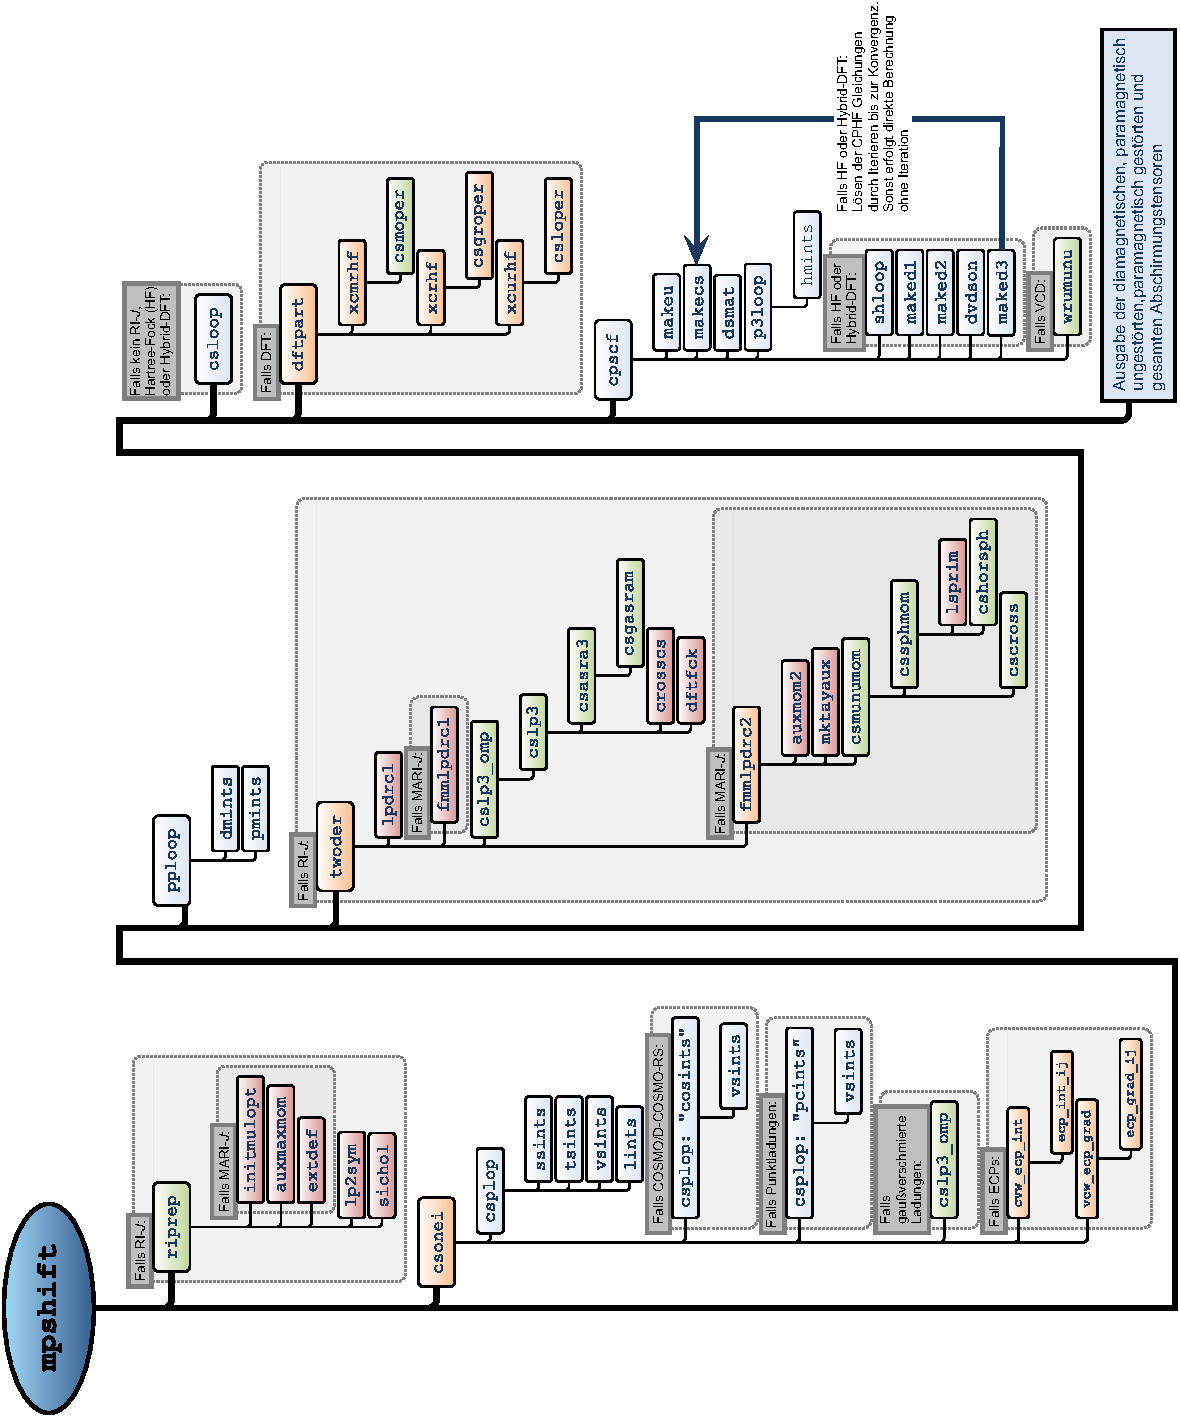
\includegraphics[width=1.1\textwidth]{mpshift_all_seitlich}
	}
	\captionsetup{figurewithin = chapter}
	\captionsetup{font=small, labelfont=bf}\caption[Neue schematische Programmstruktur des Moduls \texttt{mpshift}]{Schematische Programmstruktur des Moduls \texttt{mpshift} mit den wichtigsten Änderungen und Erweiterungen die im Rahmen der vorliegenden Arbeit durchgeführt wurden. Alte Routinen sind in blau, neue Routinen in grün, modifizierte Routinen in orange und unverändert aus anderen Modulen übertragene Routinen in rot dargestellt.}
\label{abb:neue_programmstruktur}
\end{figure}
